\documentclass[11pt,preprint]{elsarticle}

\usepackage{lmodern}
%%%% My spacing
\usepackage{setspace}
\setstretch{1.2}
\DeclareMathSizes{12}{14}{10}{10}

% Wrap around which gives all figures included the [H] command, or places it "here". This can be tedious to code in Rmarkdown.
\usepackage{float}
\let\origfigure\figure
\let\endorigfigure\endfigure
\renewenvironment{figure}[1][2] {
    \expandafter\origfigure\expandafter[H]
} {
    \endorigfigure
}

\let\origtable\table
\let\endorigtable\endtable
\renewenvironment{table}[1][2] {
    \expandafter\origtable\expandafter[H]
} {
    \endorigtable
}


\usepackage{ifxetex,ifluatex}
\usepackage{fixltx2e} % provides \textsubscript
\ifnum 0\ifxetex 1\fi\ifluatex 1\fi=0 % if pdftex
  \usepackage[T1]{fontenc}
  \usepackage[utf8]{inputenc}
\else % if luatex or xelatex
  \ifxetex
    \usepackage{mathspec}
    \usepackage{xltxtra,xunicode}
  \else
    \usepackage{fontspec}
  \fi
  \defaultfontfeatures{Mapping=tex-text,Scale=MatchLowercase}
  \newcommand{\euro}{€}
\fi

\usepackage{amssymb, amsmath, amsthm, amsfonts}

\def\bibsection{\section*{References}} %%% Make "References" appear before bibliography


\usepackage[numbers]{natbib}

\usepackage{longtable}
\usepackage[margin=2.3cm,bottom=2cm,top=2.5cm, includefoot]{geometry}
\usepackage{fancyhdr}
\usepackage[bottom, hang, flushmargin]{footmisc}
\usepackage{graphicx}
\numberwithin{equation}{section}
\numberwithin{figure}{section}
\numberwithin{table}{section}
\setlength{\parindent}{0cm}
\setlength{\parskip}{1.3ex plus 0.5ex minus 0.3ex}
\usepackage{textcomp}
\renewcommand{\headrulewidth}{0pt}

\usepackage{array}
\newcolumntype{x}[1]{>{\centering\arraybackslash\hspace{0pt}}p{#1}}

%%%%  Remove the "preprint submitted to" part. Don't worry about this either, it just looks better without it:
\journal{Journal of Finance}

 \def\tightlist{} % This allows for subbullets!

\usepackage{hyperref}
\hypersetup{breaklinks=true,
            bookmarks=true,
            colorlinks=true,
            citecolor=blue,
            urlcolor=blue,
            linkcolor=blue,
            pdfborder={0 0 0}}


% The following packages allow huxtable to work:
\usepackage{siunitx}
\usepackage{multirow}
\usepackage{hhline}
\usepackage{calc}
\usepackage{tabularx}
\usepackage{booktabs}
\usepackage{caption}


\newenvironment{columns}[1][]{}{}

\newenvironment{column}[1]{\begin{minipage}{#1}\ignorespaces}{%
\end{minipage}
\ifhmode\unskip\fi
\aftergroup\useignorespacesandallpars}

\def\useignorespacesandallpars#1\ignorespaces\fi{%
#1\fi\ignorespacesandallpars}

\makeatletter
\def\ignorespacesandallpars{%
  \@ifnextchar\par
    {\expandafter\ignorespacesandallpars\@gobble}%
    {}%
}
\makeatother


% definitions for citeproc citations
\NewDocumentCommand\citeproctext{}{}
\NewDocumentCommand\citeproc{mm}{%
\href{\#cite.\detokenize{#1}}{#2}\nocite{#1}}

\makeatletter
% allow citations to break across lines
\let\@cite@ofmt\@firstofone
% avoid brackets around text for \cite:
\def\@biblabel#1{}
\def\@cite#1#2{{#1\if@tempswa , #2\fi}}
\makeatother
\newlength{\cslhangindent}
\setlength{\cslhangindent}{1.5em}
\newlength{\csllabelwidth}
\setlength{\csllabelwidth}{3em}
\newenvironment{CSLReferences}[2] % #1 hanging-indent, #2 entry-spacing
{\begin{list}{}{%
	\setlength{\itemindent}{0pt}
	\setlength{\leftmargin}{0pt}
	\setlength{\parsep}{0pt}
	% turn on hanging indent if param 1 is 1
	\ifodd #1
	\setlength{\leftmargin}{\cslhangindent}
	\setlength{\itemindent}{-1\cslhangindent}
	\fi
	% set entry spacing
	\setlength{\itemsep}{#2\baselineskip}}}
{\end{list}}

\usepackage{calc}
\newcommand{\CSLBlock}[1]{\hfill\break\parbox[t]{\linewidth}{\strut\ignorespaces#1\strut}}
\newcommand{\CSLLeftMargin}[1]{\parbox[t]{\csllabelwidth}{\strut#1\strut}}
\newcommand{\CSLRightInline}[1]{\parbox[t]{\linewidth - \csllabelwidth}{\strut#1\strut}}
\newcommand{\CSLIndent}[1]{\hspace{\cslhangindent}#1}


\urlstyle{same}  % don't use monospace font for urls
\setlength{\parindent}{0pt}
\setlength{\parskip}{6pt plus 2pt minus 1pt}
\setlength{\emergencystretch}{3em}  % prevent overfull lines
\setcounter{secnumdepth}{5}

%%% Use protect on footnotes to avoid problems with footnotes in titles
\let\rmarkdownfootnote\footnote%
\def\footnote{\protect\rmarkdownfootnote}
\IfFileExists{upquote.sty}{\usepackage{upquote}}{}

%%% Include extra packages specified by user
\providecommand{\pandocbounded}[1]{#1}

%%% Hard setting column skips for reports - this ensures greater consistency and control over the length settings in the document.
%% page layout
%% paragraphs
\setlength{\baselineskip}{12pt plus 0pt minus 0pt}
\setlength{\parskip}{12pt plus 0pt minus 0pt}
\setlength{\parindent}{0pt plus 0pt minus 0pt}
%% floats
\setlength{\floatsep}{12pt plus 0 pt minus 0pt}
\setlength{\textfloatsep}{20pt plus 0pt minus 0pt}
\setlength{\intextsep}{14pt plus 0pt minus 0pt}
\setlength{\dbltextfloatsep}{20pt plus 0pt minus 0pt}
\setlength{\dblfloatsep}{14pt plus 0pt minus 0pt}
%% maths
\setlength{\abovedisplayskip}{12pt plus 0pt minus 0pt}
\setlength{\belowdisplayskip}{12pt plus 0pt minus 0pt}
%% lists
\setlength{\topsep}{10pt plus 0pt minus 0pt}
\setlength{\partopsep}{3pt plus 0pt minus 0pt}
\setlength{\itemsep}{5pt plus 0pt minus 0pt}
\setlength{\labelsep}{8mm plus 0mm minus 0mm}
\setlength{\parsep}{\the\parskip}
\setlength{\listparindent}{\the\parindent}
%% verbatim
\setlength{\fboxsep}{5pt plus 0pt minus 0pt}



\begin{document}



\begin{frontmatter}  %

\title{Netflix}

% Set to FALSE if wanting to remove title (for submission)




\author[Add1]{Anya Nash}
\ead{25051911@sun.ac.za}





\address[Add1]{Stellenbosch University, Stellenbosch, South Africa}

\cortext[cor]{Corresponding author: Anya Nash}


\vspace{1cm}





\vspace{0.5cm}

\end{frontmatter}

\setcounter{footnote}{0}



%________________________
% Header and Footers
%%%%%%%%%%%%%%%%%%%%%%%%%%%%%%%%%
\pagestyle{fancy}
\chead{}
\rhead{}
\lfoot{}
\rfoot{}
\lhead{}
%\rfoot{\footnotesize Page \thepage } % "e.g. Page 2"
\cfoot{}

%\setlength\headheight{30pt}
%%%%%%%%%%%%%%%%%%%%%%%%%%%%%%%%%
%________________________

\headsep 35pt % So that header does not go over title




\subsection{Summary of the Top 10 Netflix Content-Producing
Countries}\label{summary-of-the-top-10-netflix-content-producing-countries}

\pandocbounded{
\includegraphics[keepaspectratio]{25051911_Question_4_files/figure-latex/unnamed-chunk-4-1.pdf}}

As seen in the graph above, the US produces by far the most content for
Netflix. The next two highest countries are India and Great Britain.

\subsection{Relationship Between Movie TMDB Score and
Runtime}\label{relationship-between-movie-tmdb-score-and-runtime}

The scatter plot below shows the relationship between TMDB score and
runtime, by genre. As shown by the graph below, there is a very weak
relationship between TMDB score and runtime. Interestingly, though,
comedies, documentations and dramas have a somewhat similar TMDB score,
but the runtime for comedies and documentations is, on average, shorter
than the runtime of dramas. Romances and thrillers tend to have lower
scores than the aforementioned genres.


\includegraphics[width=1\linewidth]{25051911_Question_4_files/figure-latex/unnamed-chunk-5-1}

\subsection{Average TMDB Popularity of movies over time by genre and
country}\label{average-tmdb-popularity-of-movies-over-time-by-genre-and-country}

The graphs below plot the average TMDB popularity by genre and country
over time. The countries that produce the most Netflix movies are
plotted (individually) and only the top 6 genres per country are
included.

\subsubsection{US}\label{us}

As seen in the graph below, the top 6 genres for production in the US
are: comedy, drama, romance, documentation, horror and thriller. The
popularity of dramas and thrillers has increased exponentially since
2020. Therefore, it would be a good decision to focus on streaming
dramas and thrillers produced in the US.


\includegraphics[width=1\linewidth]{25051911_Question_4_files/figure-latex/unnamed-chunk-6-1}

\subsubsection{India}\label{india}

As seen in the graph below, the top 6 genres for production in India
are: comedy, drama, romance, action, crime and thriller. The popularity
of actions and comedies has increased exponentially since the late
2010s. Therefore, it would be a good decision to focus on streaming
actions and comedies produced in India.


\includegraphics[width=1\linewidth]{25051911_Question_4_files/figure-latex/unnamed-chunk-7-1}

\subsubsection{Great Britain}\label{great-britain}

As seen in the graph below, the top 6 genres for production in Great
Britain are: comedy, drama, romance, action, documentation and thriller.
The popularity of actions and documentations has increased slightly
since 2020. Therefore, it would be a good decision to focus on streaming
actions and documentations produced in Great Britain. I would be
hesitant to focus on streaming thrillers from Great Britain because,
despite increasing exponentially in 2020, their popularity appears to be
on a heavy downward trend, so it woud be a riskier investment.


\includegraphics[width=1\linewidth]{25051911_Question_4_files/figure-latex/unnamed-chunk-8-1}

\subsubsection{France}\label{france}

As seen in the graph below, the top 6 genres for production in France
are: comedy, drama, documentation, action, crime and thriller. The
popularity of thrillers and crime has increased exponentially since
2020. Therefore, it would be a good decision to focus on streaming
thrillers and crime produced in France.


\includegraphics[width=1\linewidth]{25051911_Question_4_files/figure-latex/unnamed-chunk-9-1}

\subsubsection{Canada}\label{canada}

As seen in the graph below, the top 6 genres for production in Canada
are: animation, documentation, fantasy, comedy, drama and thriller. The
popularity of fantasies, comedies and dramas have increased
exponentially since the late 2010s. Therefore, it would be a good
decision to focus on streaming fantasies, comedies and dramas produced
in Canada.

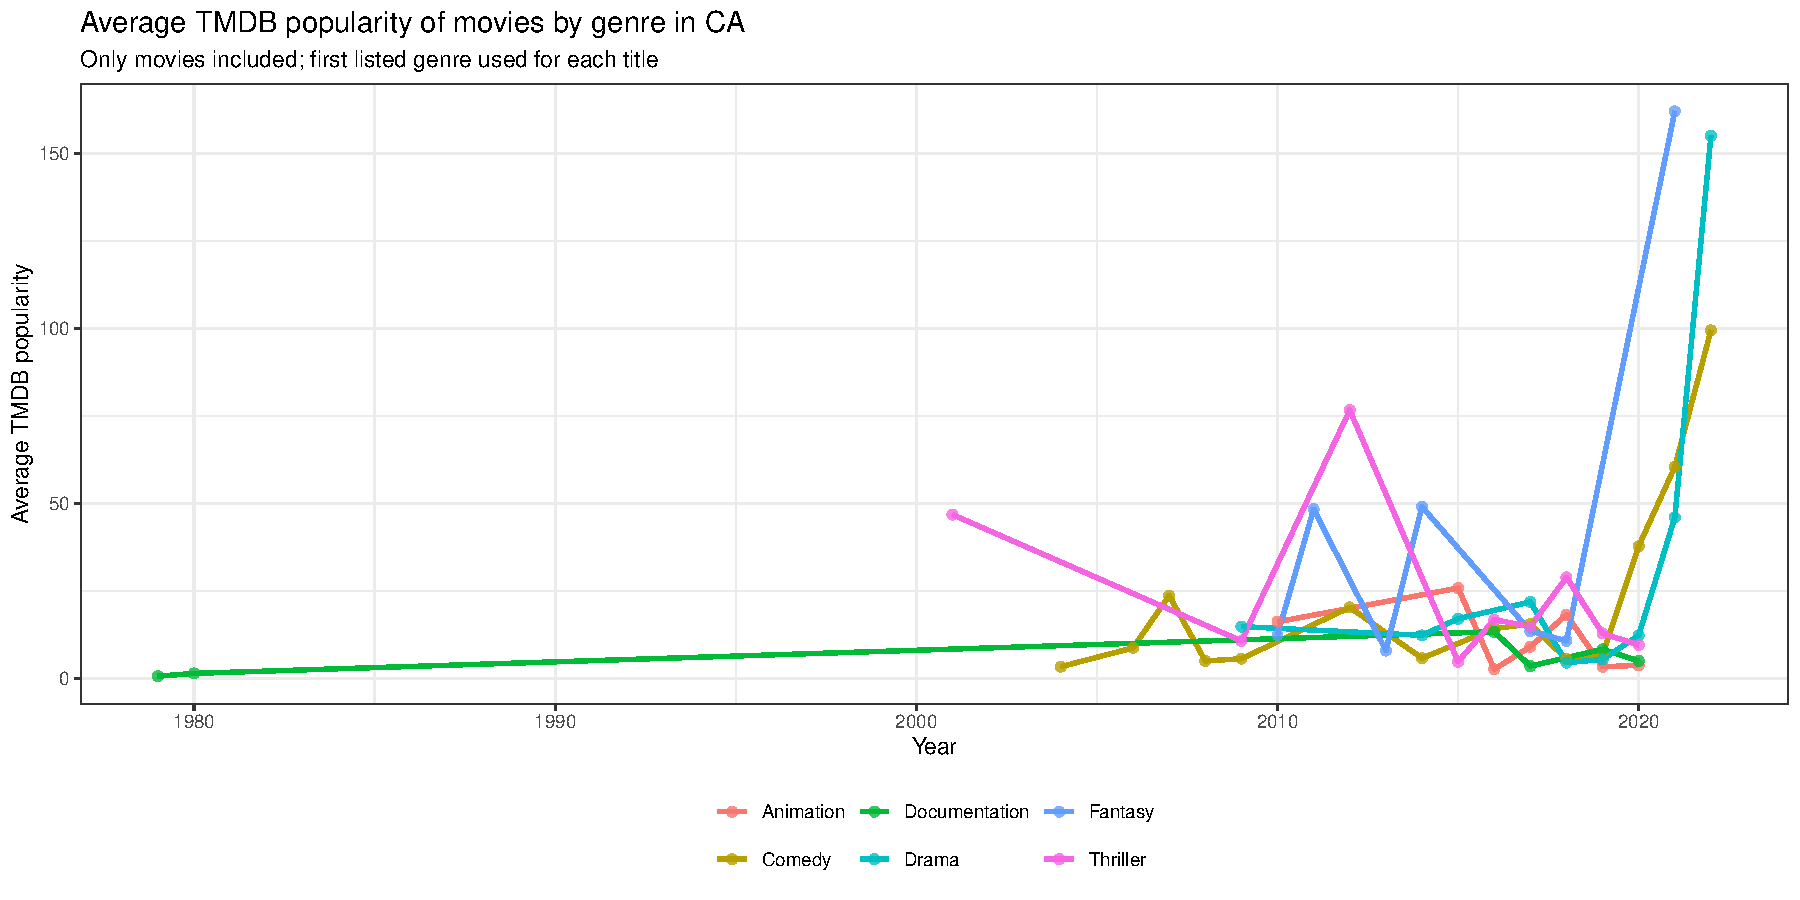
\includegraphics[width=1\linewidth]{25051911_Question_4_files/figure-latex/unnamed-chunk-10-1}

\subsubsection{Overall Recommendations}\label{overall-recommendations}

Therefore, my advice would be to invest in streaming the following
genres of movies produced in the following countries:

\begin{itemize}
\tightlist
\item
  Drama: US
\item
  Thriller: France (and maybe the US as well)
\item
  Comedy: India
\item
  Action: India (and maybe Great Britain as well)
\item
  Documentation: France
\item
  Fantasy: Canada
\item
  Drama: Canada
\end{itemize}

I would start off being a bit cautious of streaming movies that have the
genres because there is no obvious upward trend in any of the countries
analysed:

\begin{itemize}
\tightlist
\item
  Animation
\item
  Romance
\end{itemize}

\bibliography{Tex/ref}





\end{document}
